\chapter{Основное задание}

\section{Содержание проекта}

Команда разработчиков из 16 человек занимается созданием карты города на основе собственного модуля отображения. Проект должен быть завершен в течение 6 месяцев. Бюджет проекта: 50 000 рублей.

\section{Задание 1: Работа с таблицей освоенного объема}

Была задана дата отчета по заданию: 17 мая.

Были проанализированы прямые и косвенные затраты. Прямые затраты --- затраты на работу программистов и других членов команды. Они сильно больше косвенных затрат.

\begin{figure}[H]
    \begin{center}
    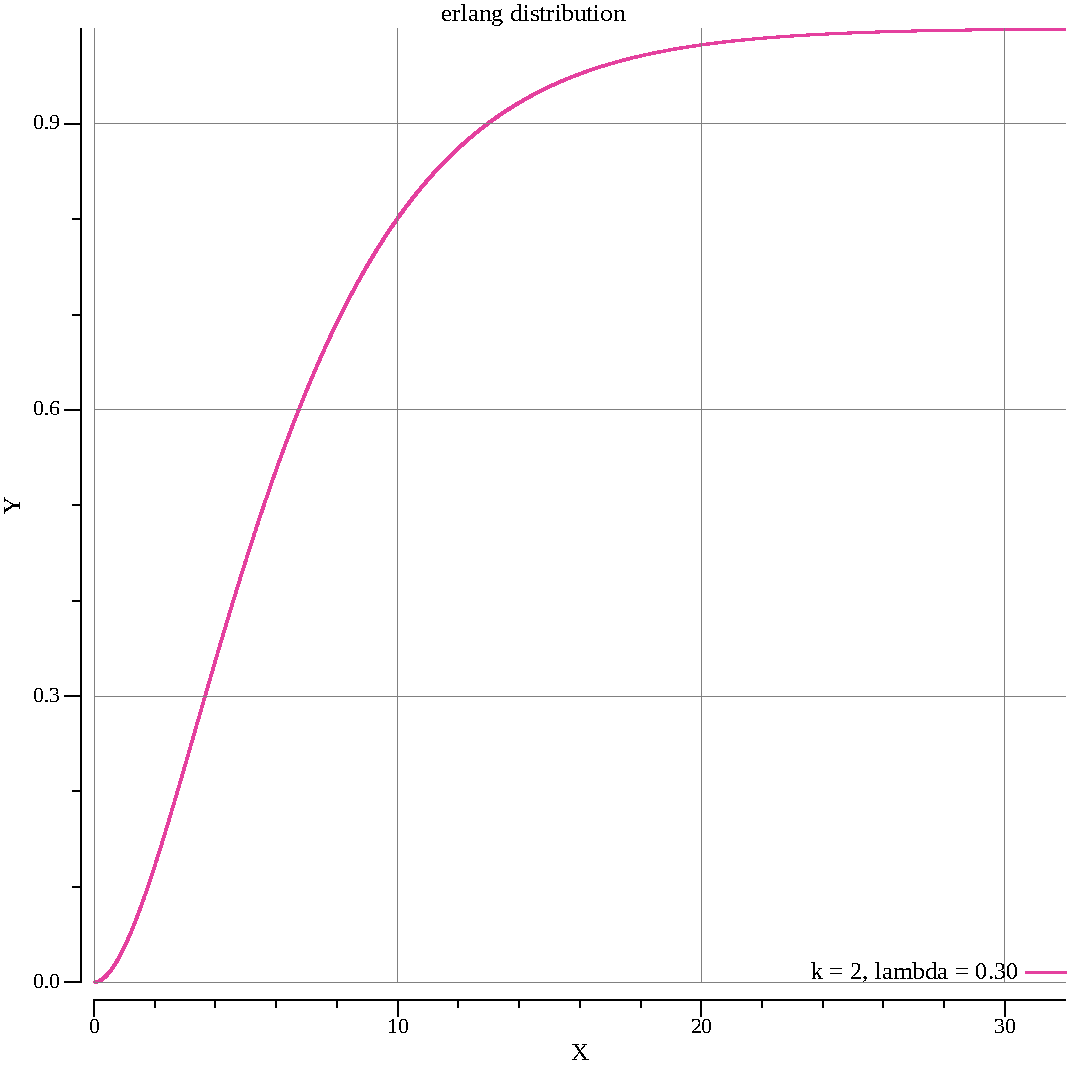
\includegraphics[width=1\linewidth]{assets/1}
    \caption{Статистика по затратам}
    \label{fig:1}
    \end{center}
\end{figure}

Была получена таблица освоенного объема.


\begin{figure}[H]
    \begin{center}
    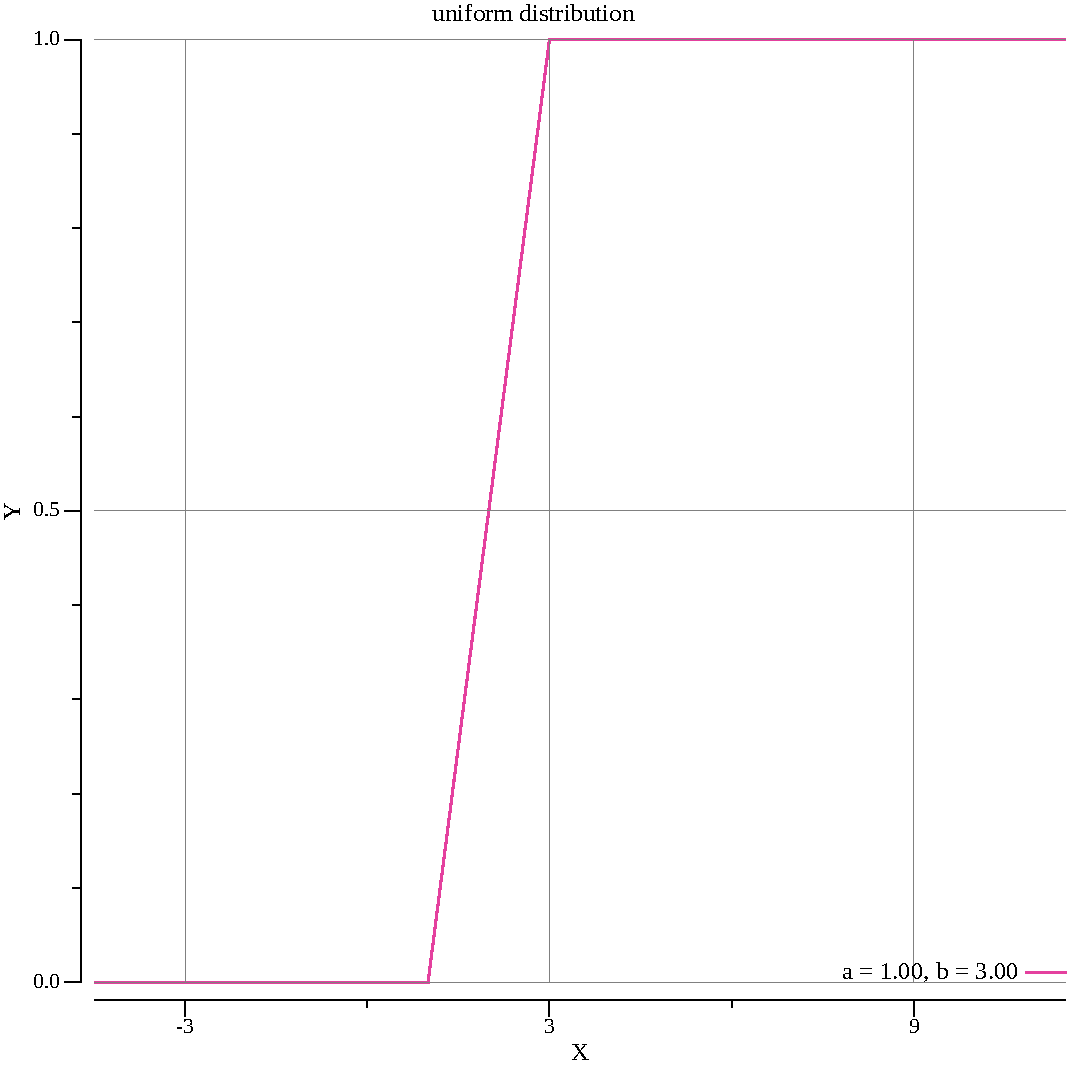
\includegraphics[width=1\linewidth]{assets/2}
    \caption{Таблица освоенного объема}
    \label{fig:2}
    \end{center}
\end{figure}

БСЗР = 26903 - затраты, которые должны были бы быть понесены на дату отчета, при объеме работ и оплате согласно базовому плану.

БСВР = 24515 - затраты, которые были бы понесены на дату отчета, при фактическом объеме работ и оплате согласно базовому плану.

ФСВР = 21997 - фактические затраты на дату отчета.

ОКП = -2387 - отклонение от календарного плана, то есть несоответствие сметы в связи с разницей объема работ.

ОПС = 2519 - отклонение по  стоимости, то есть несоответствие сметы в связи с разницей оплаты ресурсов.

ПОПЗ = 42863 - ожидаемые общие затраты, если до даты отчета учтены фактические, а после - по базовому плану.

БПЗ = 47772 - затраты по базовому плану.

ОПЗ = 4909 - отклонение по завершению, разница между базовым планом и планируемой стоимостью.

Отрицательное ОКП возникает потому, что программист 1 уходил на стажировку, а ведущий покинул проект. Это можно более детально увидеть в отрицательном ОКП в задаче про создание ядра GIS.

У создания интерфейса ОКП 277 рублей, значит оно опережает план. Опережение связано в опережением темпа в задаче 5.

Основной причиной положительного ОПС стало отсутствие затрат на сервер.

\section{Задание 2: Работа с отчетами проекта}

На рисунке представлена диаграмма затрат, сгруппированная по кварталам.
Из диаграммы видно, что руководитель проекта будет испытывать наибольшую потребность в деньгах во втором квартале. 

При этом, фактические затраты во втором квартале заметно ниже планируемых, так как из-за ухода ведущего программиста затраты на программистов стали ниже.

\begin{figure}[H]
    \begin{center}
    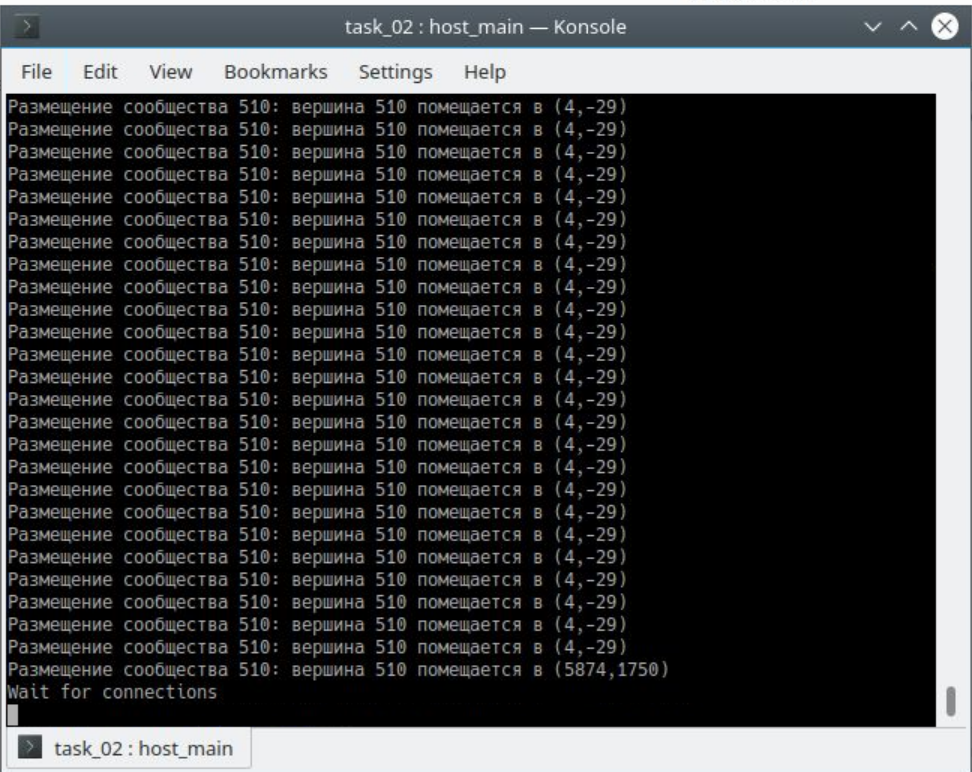
\includegraphics[width=1\linewidth]{assets/3}
    \caption{Диаграмма затрат по кварталам}
    \label{fig:3}
    \end{center}
\end{figure}

Был выведен график отклонения от бюджетной стоимости. По нему видно, что следующие задачи превышают бюджетную стоимость.

\begin{itemize}
	\item Создание интерфейса
	\item Создание ядра GIS --- дороже из-за затрат на программистов
	\item Создание мультимедиа-наполнения --- дороже из-за повышения зарплаты мультимедиа-корреспондента
	\item Тестирование сайта --- дороже из-за затрат на программистов
	\item Совещание
\end{itemize}

\begin{figure}[H]
    \begin{center}
    \includegraphics[width=1\linewidth]{assets/4}
    \caption{Отклонение от бюджетной стоимости}
    \label{fig:4}
    \end{center}
\end{figure}

\section{Задание 3: Анализ вариантов декомпозиции работ в проекте}

Был предложен альтернативный вариант декомпозиции работа в проекте, основанный на каскадной модели. В рамках него, было выделено 3 основных этапа:

\begin{enumerate}
	\item Анализ и проектирование
	\item Кодирование
	\item Тестирование
\end{enumerate}

Каждый новый этап заканчивается строго после окончания предыдущего.

В результате был получен следующий лист задач.

\begin{figure}[H]
    \begin{center}
    \includegraphics[width=1\linewidth]{assets/5}
    \caption{Задачи после декомпозиции}
    \label{fig:5}
    \end{center}
\end{figure}

Были получены следующие перегрузки по ресурсам.

\begin{enumerate}
	\item Системный аналитик --- так как одновременно на этапе анализа делает задачи "Анализ и построение структуры базы проектов" и "Анализ и проектирование ядра"
	
	\begin{figure}[H]
    \begin{center}
    \includegraphics[width=1\linewidth]{assets/6}
    \caption{Перегрузка системного аналитика}
    \label{fig:6}
    \end{center}
	\end{figure}
	
	\item Ведущий программист и программист 1 --- так как одновременно делают Создание модели ядра и создание рабочей версии ядра.
	
	\begin{figure}[H]
    \begin{center}
    \includegraphics[width=1\linewidth]{assets/7}
    \caption{Перегрузка программистов}
    \label{fig:7}
    \end{center}
	\end{figure}
	
	\item Программист 1 --- так как одновременно делает тестирование модели ядра и тестирование сайта.
	
	\begin{figure}[H]
    \begin{center}
    \includegraphics[width=1\linewidth]{assets/8}
    \caption{Перегрузка программистов}
    \label{fig:8}
    \end{center}
	\end{figure}
	
	\item Технический писатель --- так как одновременно делает написание руководства пользователя и создание справочной системы.
	
	\begin{figure}[H]
    \begin{center}
    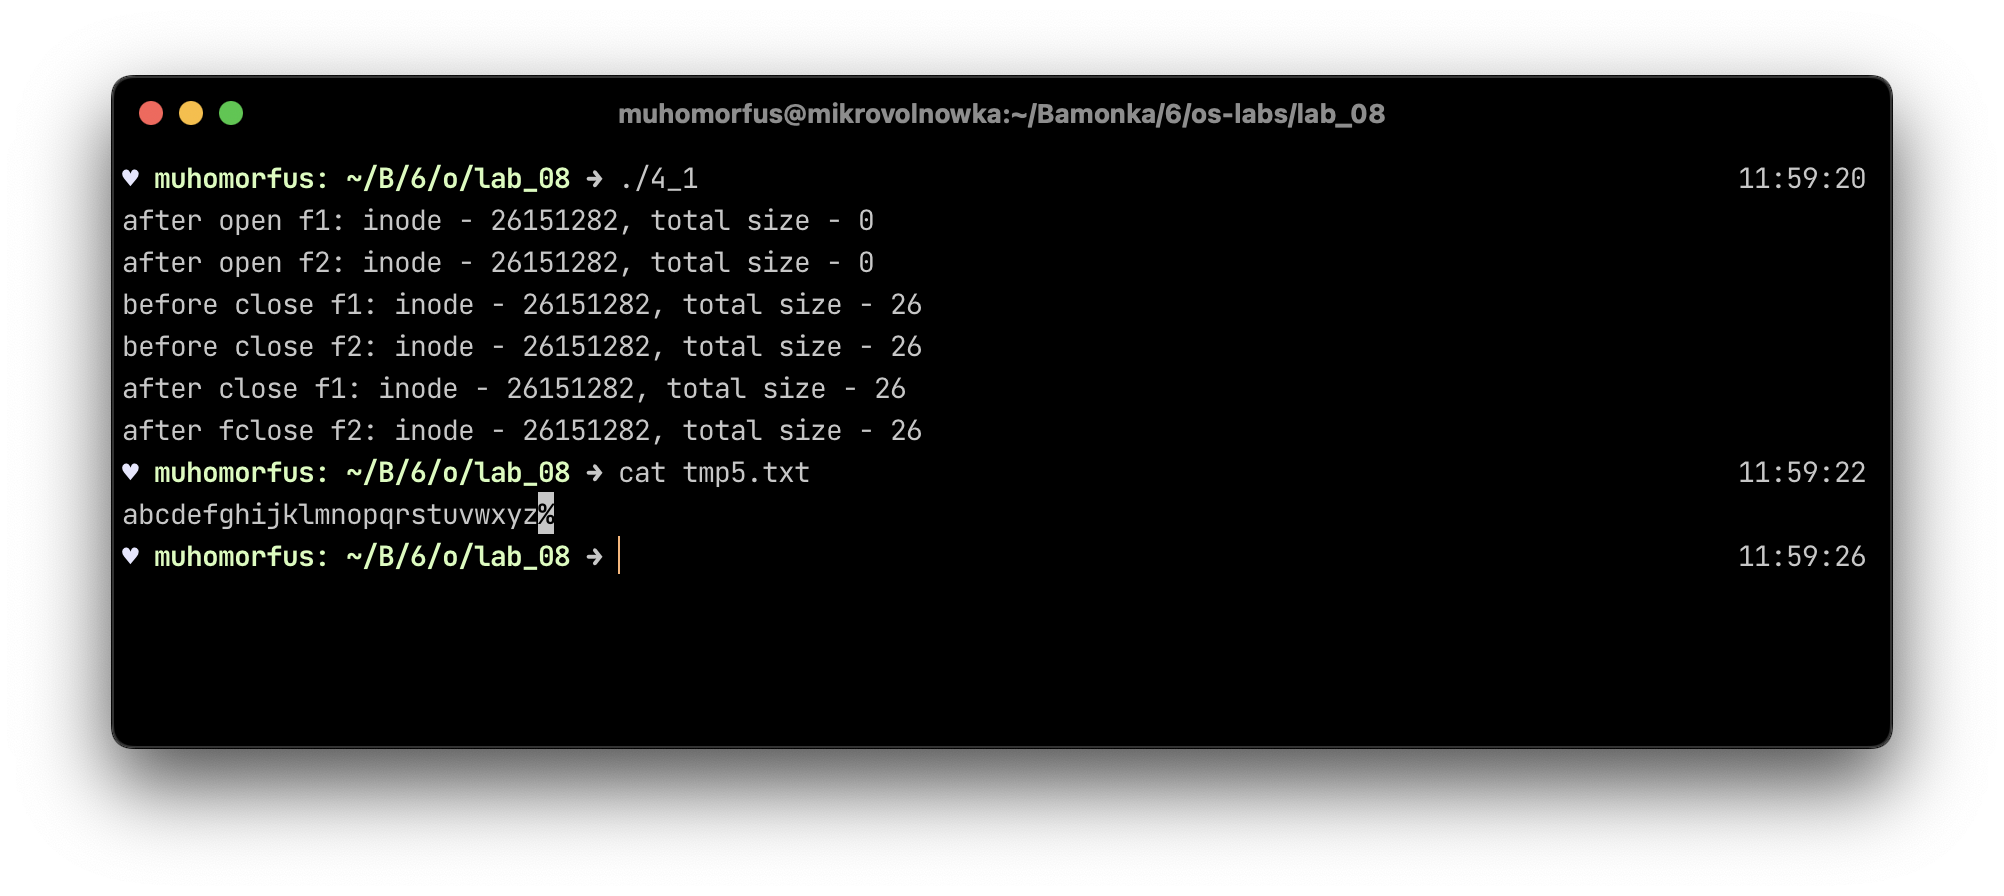
\includegraphics[width=1\linewidth]{assets/9}
    \caption{Перегрузка технического писателя}
    \label{fig:9}
    \end{center}
	\end{figure}
\end{enumerate}

Таким образом, использование каскадной модели разработки привело к перегрузкам, так как в одном этапе должна быть сосредоточено выполнение всех задач одного типа (анализ, тестирование).

После изменения декомпозиции была получена следующая статистика проекта.

\begin{figure}[H]
    \begin{center}
    \includegraphics[width=1\linewidth]{assets/10}
    \caption{Статистика}
    \label{fig:10}
    \end{center}
	\end{figure}
